%%%%%%%%%%%%%%%%%%%%%%%%%%%%%%%%%%%%%%%%%%%%%%%%%%%%%%%%%%%%%%%%%%%%%%%
%%%%%%%%%%%%%%%%%%%%%%%%%%%%%%%%%%%%%%%%%%%%%%%%%%%%%%%%%%%%%%%%%%%%%%% 
%%%%%%%%%%%       								 Preamble				         	                                                        %%%%%%%%%% 
%%%%%%%%%%%%%%%%%%%%%%%%%%%%%%%%%%%%%%%%%%%%%%%%%%%%%%%%%%%%%%%%%%%%%%% 
%%%%%%%%%%%%%%%%%%%%%%%%%%%%%%%%%%%%%%%%%%%%%%%%%%%%%%%%%%%%%%%%%%%%%%% 
\documentclass[10pt]{beamer}
\usepackage{setspace}
\usepackage{color}
\usepackage{amsmath,lmodern}
\usepackage{hyperref}
\usepackage{graphicx}
\usepackage{multirow}
\usepackage{tikz}
\usetikzlibrary{fit,shapes.misc}
\usepackage{pdflscape}
\usepackage{amsmath}
\usepackage{lscape}
\usepackage{multirow}
\usepackage{enumerate}
\usepackage{epstopdf}
\usepackage{pdfpages}
\usepackage{appendixnumberbeamer}
\usepackage{color,soul}
\usepackage{grffile}
\usepackage{float}
\usepackage{relsize}
\usepackage{tcolorbox}
\newcounter{nodemarkers}
\usepackage{tikz}
\newcommand{\toplinesmall}{%
  \tikz[remember picture,overlay] {%
    \draw[blue,thick] ([yshift=-1cm, xshift=.9cm]current page.north west)
             -- ([yshift=-1cm,xshift=3.6cm]current page.north west);}}
             
\newcommand{\toplinemedium}{%
  \tikz[remember picture,overlay] {%
    \draw[blue,thick] ([yshift=-1cm, xshift=.9cm]current page.north west)
             -- ([yshift=-1cm,xshift=6.2cm]current page.north west);}}
 
 \newcommand{\toplinelarge}{%
  \tikz[remember picture,overlay] {%
    \draw[blue,thick] ([yshift=-1cm, xshift=.9cm]current page.north west)
             -- ([yshift=-1cm,xshift=8.9cm]current page.north west);}}           
             
 \newcommand{\toplinexlarge}{%
  \tikz[remember picture,overlay] {%
    \draw[blue,thick] ([yshift=-1cm, xshift=.9cm]current page.north west)
             -- ([yshift=-1cm,xshift=12cm]current page.north west);}}                       
             
\setbeamertemplate{footline}
{
  \leavevmode%
  \hbox{%
  \begin{beamercolorbox}[wd=.333333\paperwidth,ht=2.25ex,dp=1ex,center]{author in head/foot}%
    \usebeamerfont{author in head/foot}{\textcolor{blue}{ECON311}}
  \end{beamercolorbox}%
  \begin{beamercolorbox}[wd=.333333\paperwidth,ht=2.25ex,dp=1ex,center]{title in head/foot}%
    \usebeamerfont{title in head/foot}{\textcolor{blue}{Winter 2026}}
  \end{beamercolorbox}%
  \begin{beamercolorbox}[wd=.333333\paperwidth,ht=2.25ex,dp=1ex,right]{date in head/foot}%
    \usebeamerfont{date in head/foot}{\textcolor{blue}{Lecture 18 \: \: \: \: \: \: \: }
    \insertframenumber{} / \inserttotalframenumber\hspace*{2ex}} 
  \end{beamercolorbox}}%
  \vskip0pt%
}
\newtheorem{proposition}[theorem]{Proposition}

\newcommand\marktopleft[1]{%
    \tikz[overlay,remember picture] 
        \node (marker-#1-a) at (-0.2,1.2ex) {};%
}
\newcommand\markbottomright[1]{%
    \tikz[overlay,remember picture] 
        \node (marker-#1-b) at (0.16,-1ex) {};%
    \tikz[overlay,remember picture,thick,inner sep=4pt]
        \node[draw,rectangle,rounded corners, blue, fit=(marker-#1-a.center) (marker-#1-b.center)] {};%
}

\setbeamertemplate{caption}{\raggedright\insertcaption\par}
\setbeamertemplate{itemize items}[ball]
\setbeamertemplate{itemize subitem}[triangle]
\setbeamertemplate{itemize subsubitem}[triangle]
\tcbset{colframe=white,colback=white,nobeforeafter}
\beamertemplatenavigationsymbolsempty
\addtobeamertemplate{frametitle}{\vspace*{0.19cm}}{\vspace*{0cm}}


%%%%%%%%%%%%%%%%%%%%%%%%%%%%%%%%%%%%%%%%%%%%%%%%%%%%%%%%%%%%%%%%%%%%%%%
%%%%%%%%%%%%%%%%%%%%%%%%%%%%%%%%%%%%%%%%%%%%%%%%%%%%%%%%%%%%%%%%%%%%%%% 
%%%%%%%%%  									    Define Title									                                       %%%%%%%%%
%%%%%%%%%%%%%%%%%%%%%%%%%%%%%%%%%%%%%%%%%%%%%%%%%%%%%%%%%%%%%%%%%%%%%%%
%%%%%%%%%%%%%%%%%%%%%%%%%%%%%%%%%%%%%%%%%%%%%%%%%%%%%%%%%%%%%%%%%%%%%%% 
\title{ECON 311} 
\author{Lecture 18: AS-AD Model, part II}
\date{}
\AtBeginSection[]
{
 \begin{frame}<beamer>
 \tableofcontents[currentsection]
 \end{frame}
}
%%%%%%%%%%%%%%%%%%%%%%%%%%%%%%%%%%%%%%%%%%%%%%%%%%%%%%%%%%%%%%%%%%%%%%%
%%%%%%%%%%%%%%%%%%%%%%%%%%%%%%%%%%%%%%%%%%%%%%%%%%%%%%%%%%%%%%%%%%%%%%% 
%%%%%%%% 						     				Document								                                                %%%%%%%%
%%%%%%%%%%%%%%%%%%%%%%%%%%%%%%%%%%%%%%%%%%%%%%%%%%%%%%%%%%%%%%%%%%%%%%%
%%%%%%%%%%%%%%%%%%%%%%%%%%%%%%%%%%%%%%%%%%%%%%%%%%%%%%%%%%%%%%%%%%%%%%% 
\begin{document}
\setbeamercovered{transparent}

\begin{frame}
\maketitle
\end{frame}

\section{Using the AS-AD Model}



\begin{frame}
\frametitle{\: \: \: Cost-push Shock}
\toplinemedium
\begin{figure}
\centering
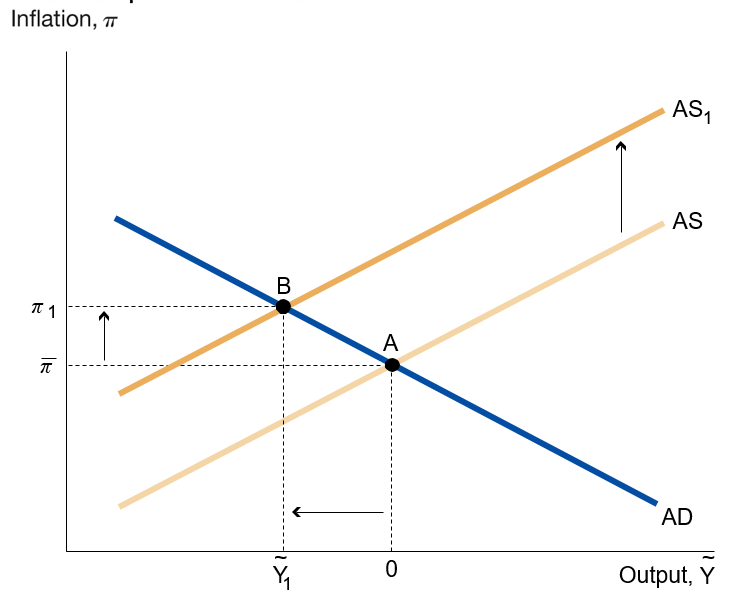
\includegraphics[scale=.45]{AS_AD_inflation}
\end{figure}
\end{frame}

\begin{frame}
\frametitle{\: \: \: Inflation Shock}
\toplinemedium
\begin{figure}
\centering
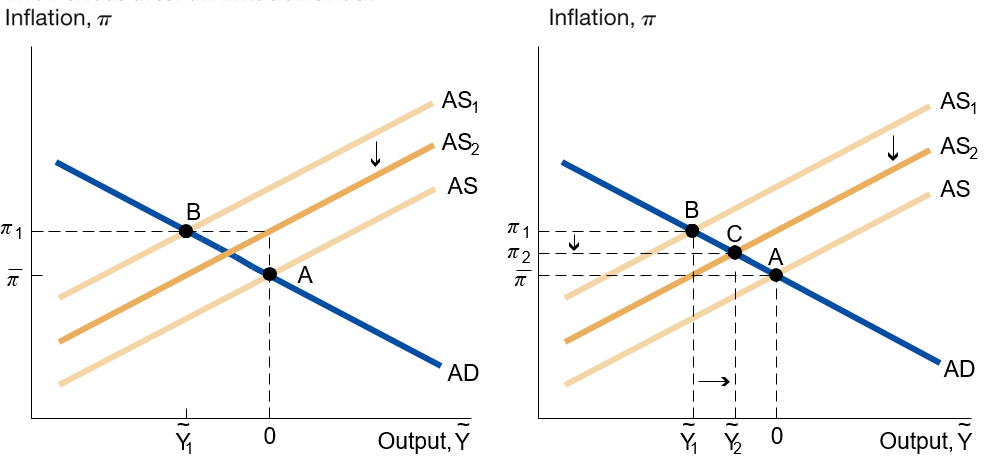
\includegraphics[scale=.45]{AS_AD_inflation_2}
\end{figure}
\end{frame}

\begin{frame}
\frametitle{\: \: \: Cost-push Shock}
\toplinemedium
\begin{figure}
\centering
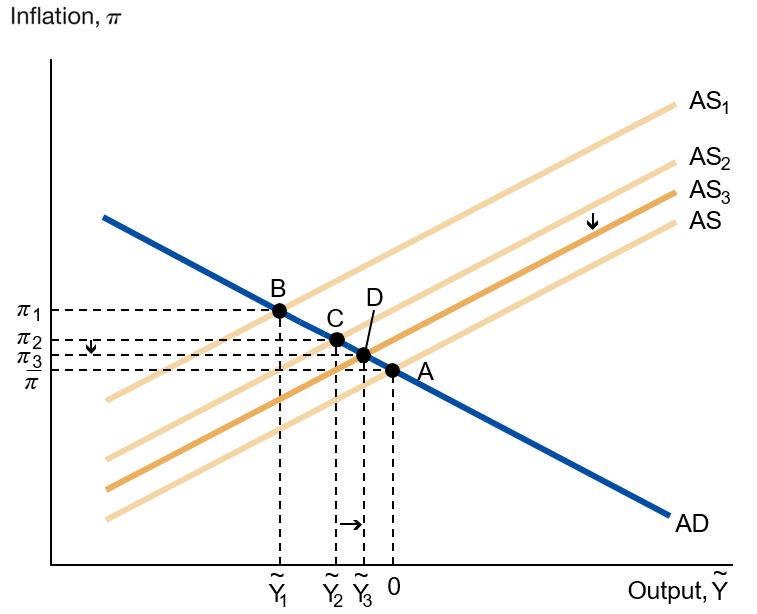
\includegraphics[scale=.45]{AS_AD_inflation_3}
\end{figure}
\end{frame}

\begin{frame}
\frametitle{\: \: \: Cost-push Shock}
\toplinemedium
\begin{figure}
\centering
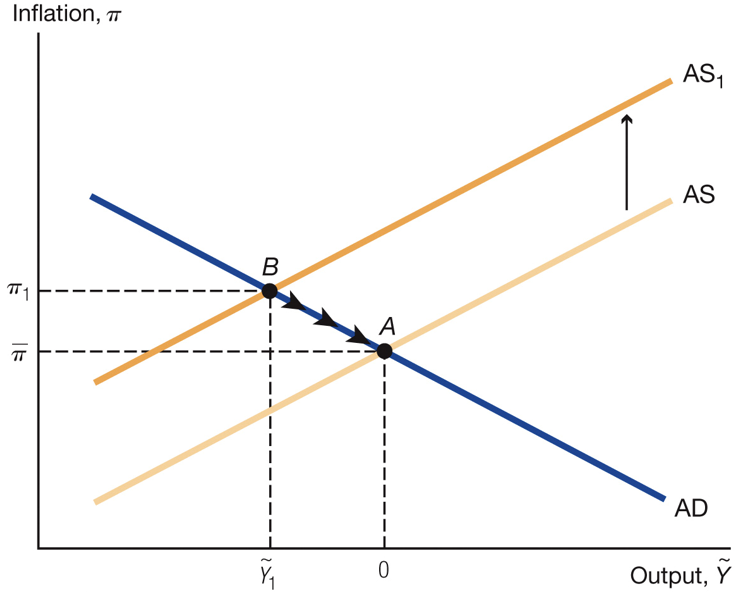
\includegraphics[scale=.45]{AS_AD_inflation_4}
\end{figure}
\end{frame}


\begin{frame}
\frametitle{\: \: \: One Period Demand Shock}
\toplinemedium
\begin{figure}
\centering
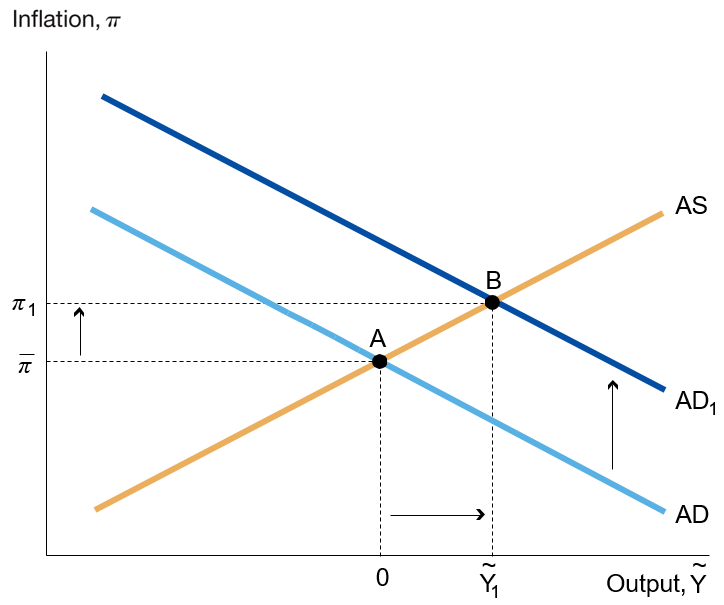
\includegraphics[scale=.45]{demand_shock_1}
\end{figure}
\end{frame}

\begin{frame}
\frametitle{\: \: \: One Period Demand Shock}
\toplinemedium
\begin{figure}
\centering
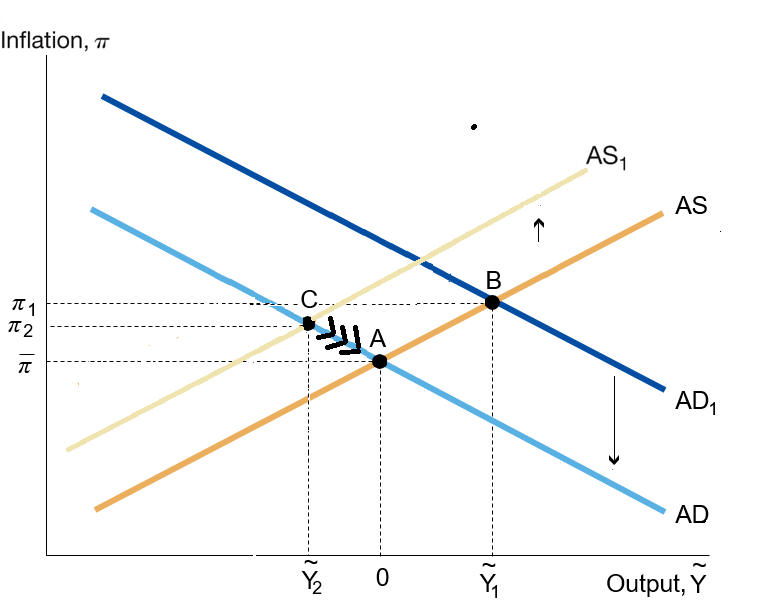
\includegraphics[scale=.45]{demand_shock_2}
\end{figure}
\end{frame}


\begin{frame}
\frametitle{\: \: \: Multiple Period Demand Shock}
\toplinemedium
\begin{figure}
\centering
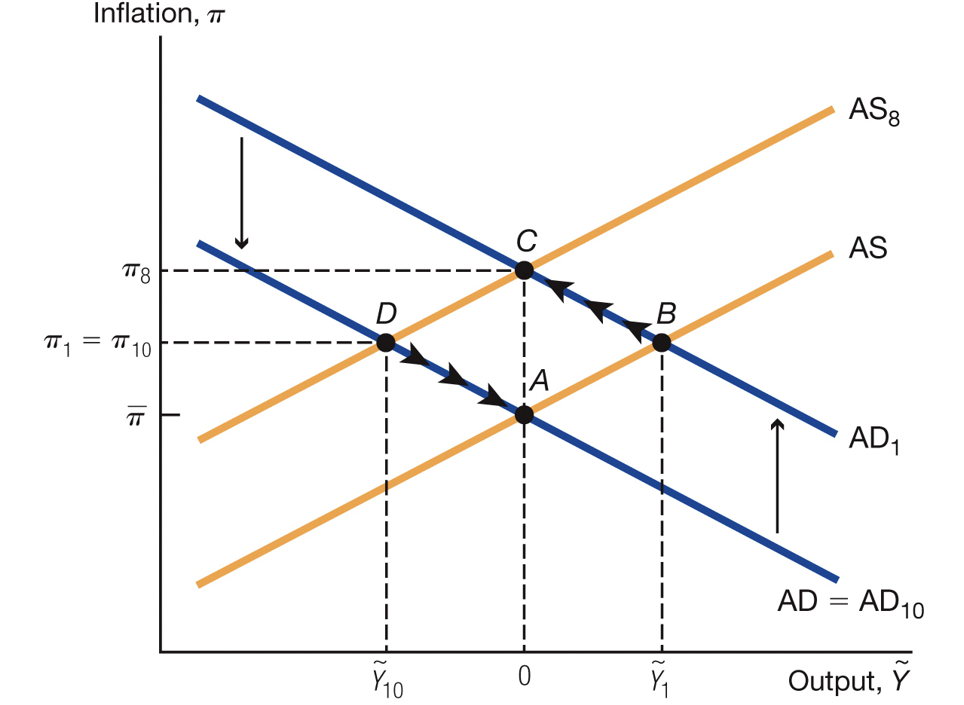
\includegraphics[scale=.35]{demand_shock_3}
\end{figure}
\end{frame}


\begin{frame}
\frametitle{\: \: \: Phase diagram cost push and demand shocks}
\toplinexlarge
\begin{figure}
\centering
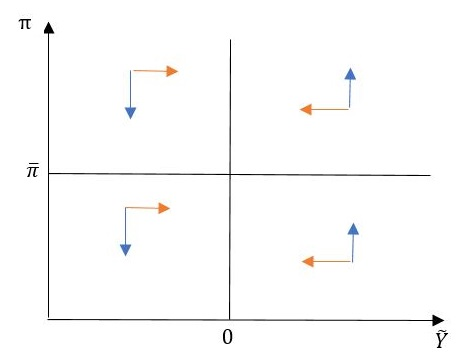
\includegraphics[scale=.67]{phase_diagram}
\end{figure}
\end{frame}



\begin{frame}
\frametitle{\: \: \: Empirical Evidence}
\toplinemedium
\begin{figure}
\centering
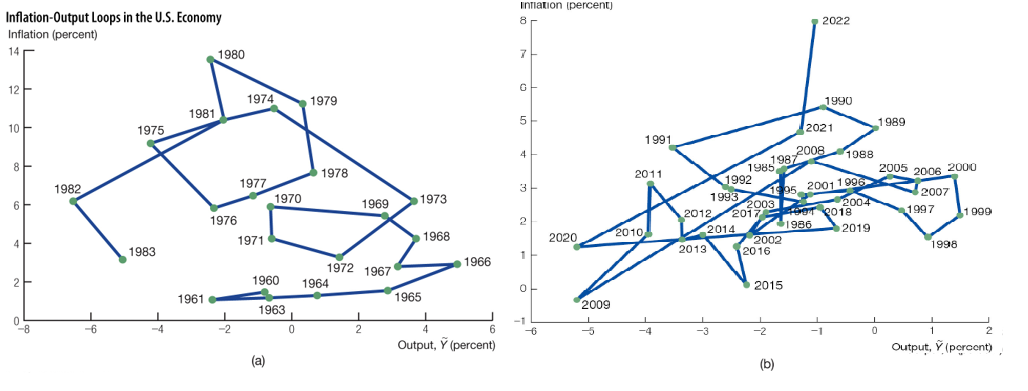
\includegraphics[scale=.4]{empirics}
\end{figure}
\end{frame}

\begin{frame}
\frametitle{\: \: \: Rules vs. Discretion}
\toplinemedium
\begin{itemize}
\item Explicit Policy Rules:
\vspace{0.1in}
\begin{itemize}
\item (pros) Help anchor inflation expectations and maintain a stable inflation environment where shocks are deflected quickly
\vspace{0.1in}
\item (cons) To work, policy rules must be credible, and, therefore, provide little flexibility to deviate from targets
\end{itemize}
\vspace{0.1in}
\item Discretionary Monetary Policy:
\begin{itemize}
\vspace{0.1in}
\item (pros) Provides flexibility to pursue expansionary economic policy
\vspace{0.1in}
\item (cons) Shocks can be very disruptive as inflation pressures do not dissipate quickly
\end{itemize}
\vspace{0.1in}
\item It is extremely important that, in Modern Economies, CBs are independent from the government in power
\end{itemize}
\end{frame}

\section{Financial Crisis of 2008}

\begin{frame}
\frametitle{\: \: \: Great Recession}
\toplinemedium
\begin{figure}
\centering
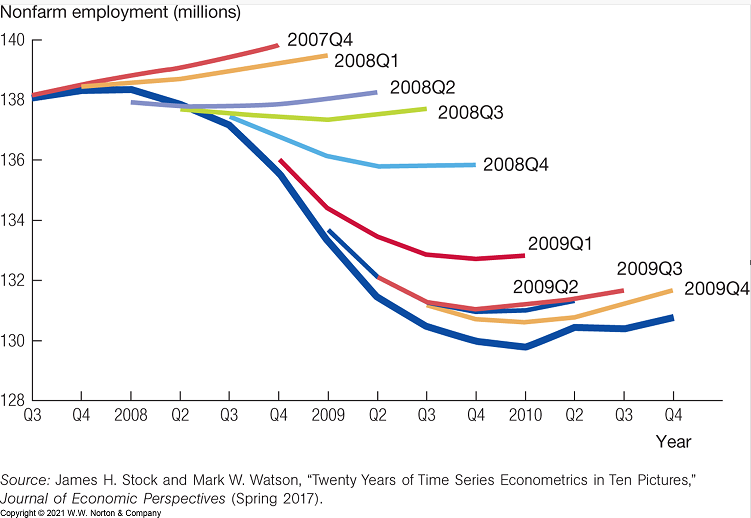
\includegraphics[scale=.5]{2008_Financial_Crisis}
\end{figure}
\end{frame}

\begin{frame}
\frametitle{\: \: \: Great Recession: Shocks}
\toplinemedium
Sequence of events that led to the crisis
\begin{itemize}
\item Global Savings Glut
\only<1>{
\begin{itemize}
\vspace{0.1in}
\item In 1996, developing countries borrowed from the rest of the world.
\vspace{0.1in}
\item In 2003, developing countries were saving a net $\$205$ billion into the world’s capital markets.
\vspace{0.1in}
\item Most of these savings enter the US market 
\vspace{0.1in}
\end{itemize}}
\item Housing Market and Subprime lending
\only<2>{
\begin{itemize}
\vspace{0.1in}
\item Free Money led to subprime lending in housing markets through a variety of financial instruments deemed as "safe" assets (securatization)
\vspace{0.1in}
\item The system worked as long as housing prices were increasing
\vspace{0.1in}
\end{itemize}}
\item Rise interest rates and decrease housing prices 
\only<3>{
\begin{itemize}
\vspace{0.1in}
\item Between 2004 and 2006, the Fed raised its interest rate from $1.25\%$ to $5.25\%$ $\Rightarrow$ Higher interest rates ($>$teaser) for subprime debtors 
\vspace{0.1in}
\item From mid-2006 to the beginning of 2012, Housing prices plummeted by $36\%$ (bubble burst)
\vspace{0.1in}
\end{itemize}}
\item Oil Prices
\only<4>{\begin{itemize}
\vspace{0.1in}
\item In 2002, oil was about $\$20$ per barrel.
\vspace{0.1in}
\item During the summer of 2008, prices peaked at $\$140$ per barrel.
\end{itemize} }
\end{itemize}
\end{frame}

\begin{frame}
\frametitle{\: \: \: Great Recession}
\toplinemedium
\begin{figure}
\centering
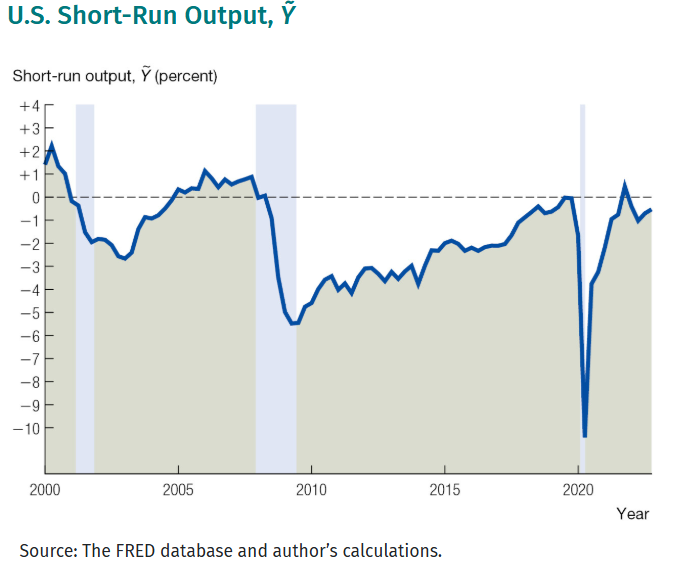
\includegraphics[scale=.58]{2008_output}
\end{figure}
\end{frame}

\begin{frame}
\frametitle{\: \: \: Great Recession}
\toplinemedium
\begin{figure}
\centering
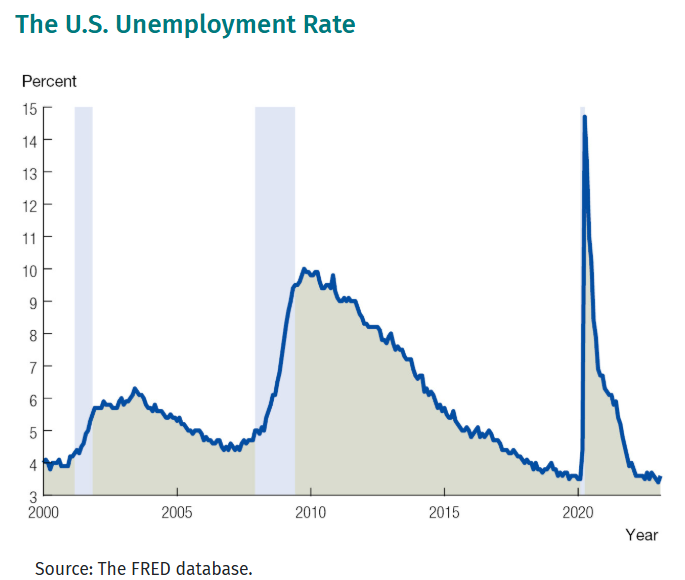
\includegraphics[scale=.5]{unemp_2008}
\end{figure}
\end{frame}

\begin{frame}
\frametitle{\: \: \: Great Recession}
\toplinemedium
\begin{figure}
\centering
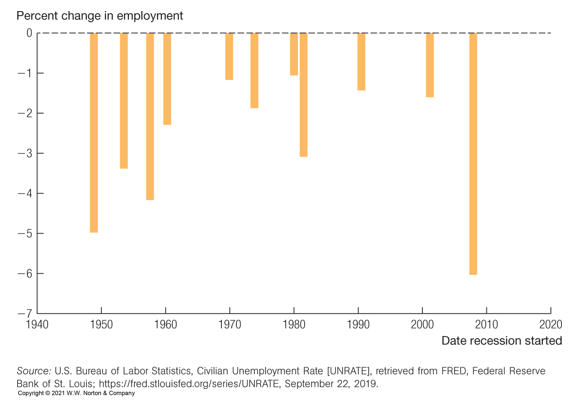
\includegraphics[scale=.58]{unemp_2008_2}
\end{figure}
\end{frame}

\begin{frame}
\frametitle{\: \: \: Great Recession}
\toplinemedium
\begin{figure}
\centering
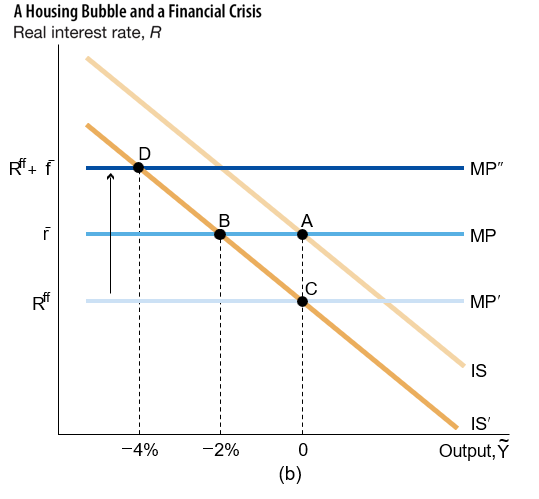
\includegraphics[scale=.58]{2008_MP}
\end{figure}
\end{frame}

\begin{frame}
\frametitle{\: \: \: Great Recession}
\toplinemedium
\begin{figure}
\centering
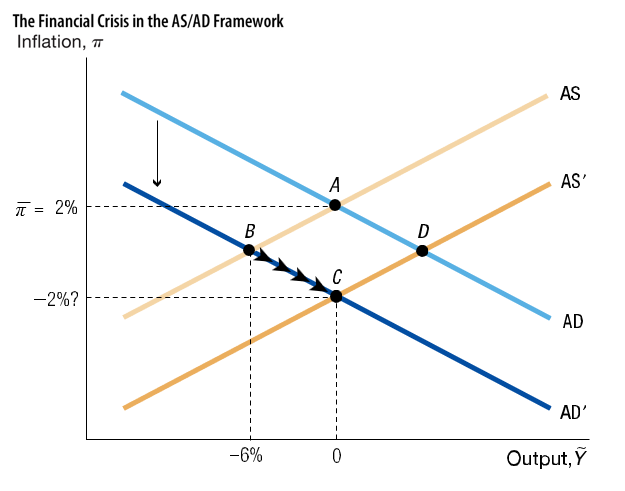
\includegraphics[scale=.58]{2008_AD}
\end{figure}
\end{frame}


\end{document}
